\section{Cost variables}
Computing costs occur for blockchain applications, and because the blockchain is decentralized, there needs to be a reward system for the people that provide the service of confirming the transactions.
Therefore, a blockchain application can be significantly more expensive than a comparable centralized service.

The costs of a single transaction on the Ethereum blockchain is dependant on at least 5 variable factors. 

When a node wants to submit a transaction to the blockchain or create a new contract, a certain amount of {'}gas{'} has to be offered to so called {'}block miners{'}. For the purpose of a cost model, gas is as a real money cost and should be treated as a currency.

The 5 variable factors are:

\textbf{1. The operations being done:} Each smart contract consists under the hood of a set of 31 possible assembly operations \cite{YellowPaper}. Such operations can for example be \texttt{ADD} which adds numbers together or \texttt{SHA3} which generates a hash.

\par
\textbf{2. The gas costs assigned to those operations:} Referred to as the 'Fee schedule', in the Ethereum yellow paper \cite{YellowPaper} a fee for each operation is defined. For example, a transaction costs 21000 gas and a SHA3 hash operation costs 30 gas.

In general, it can be stated that more complicated contracts and transactions cost more gas. Interestingly, the different gas prices for operations are not necessarily proportional of the actual computational work needed, but were set by the Ethereum developers and accepted by the majority of Ethereum users.

Because of the non-proportionality, some assembly instructions will change their gas prices in the future for rebalancing purposes when and if the majority of nodes upgrade to the Metropolis hard fork, the next version of Ethereum. For example, the cost of a CALL operation will be increased from 700 to 4000 gas with the Metropolis upgrade \cite{EIP150}.
The fact that gas prices can change is the reason the two above mentioned variables are separated in this model.

In summary, gas prices are determined by the community and are heavily influenced by the Ethereum Foundation. Gas prices can change over time, so that the very same transaction can cost more or less gas depending on the time when it is committed.

\par
\textbf{3. Gas price and desired speed:} 1 'gas' corresponds to a specific amount of Ether. The price of a gas is formed by the users of the Ethereum network and unlike the previously mentioned gas fee schedule, the gas-to-ether conversion rate is not hardcoded into the Ethereum, but determined by the users dynamically.

Each Ethereum client 'signals' a gas price. The default configuration of go-ethereum \cite{DefaultGoEthereumConfiguration}, which is the standard implementation for Ethereum, sets a gas price of 20 shannon\footnote{ Shannon is $10^{-9}$ Ether. A shannon is also known as a 'Gwei'. In the context of gas prices, 'shannon' is more commonly used.}, although it is configurable. When the gas price is set to 20 shannon in a miners client, the miner will only mine transactions that offer a gas price of 20 shannon or more. When the gas price is set to 20 shannon in a client, the client will offer this amount for a transaction and on the other hand mine transactions that offer at least this amount.

The average gas price chart from etherscan.io \cite{AverageGasPrice} shows that the clients of the network mostly go with the default configuration value, with the average price being 23 shannon.

The reason that the real average gas price is slightly higher than 20 shannon is because clients can voluntarily offer a higher price for a transaction, like for example a gas price of 24 shannon. This has the effect that the transaction will be mined faster.

The mechanics of transaction mining are similar to those of a stock market: If a stock is worth 100 USD, is being actively traded on an exchange and a buyer is willing to buy the stock at an overvalued price of for example 102 USD, his offer will jump to the top of the order book and will be filled the quickest. In Ethereum, the best gas price offers will be mined first. For our application, it could be desirable to pay a premium for faster transaction mining.

The default price of gas is debated in the Ethereum community and was already changed once in March 2016 when the price for Ether soared. The gas price was then reduced from 50 shannon to 20 shannon. Now that the Ether price has reached a different magnitude, another correction might be included in the next hard fork. At the time of writing, the gas price equilibrium would be 16 shannon according to the calculation from etherchain.org.

On May 7th 2017, ethgasstation.info announced \cite{ETHGasStationAnnouncement} that 10\% of the network hashpower is accepting a gas price of only 2 shannon. The site is promoting lower gas prices and is encouraging Ethereum users to change the settings to allow lower gas prices. According to the same site, for a transaction that offers 2 shannon per gas, the mean transaction confirmation time is 119 seconds. For 20 shannon and 28 shannon, the average transaction confirmation time is 44 and 30 seconds respectively.

\begin{figure}[H]
\centering
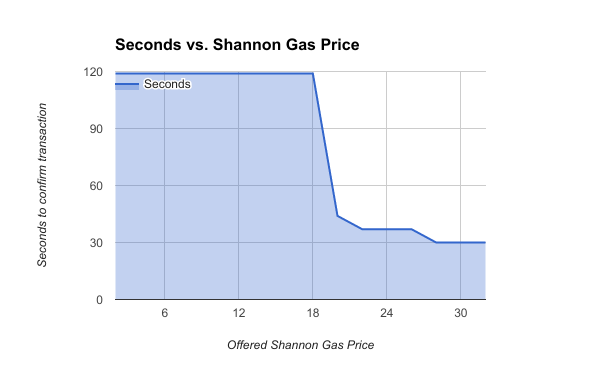
\includegraphics[width=0.85\textwidth]{gas-vs-transaction-time.png}
\caption{Average time until transaction is confirmed. Made with data from ethgasstation.info on May 8th.}
\label{fig:gas}
\end{figure}

In Figure ~\ref{fig:gas}, it can be seen that a node that offers a higher reward for a transaction will get confirmed 4 times faster on average. The client has to decide based on that information, how much gas it wants to offer.

\textbf{4. Price of Ether:} Ether can either be mined or can be purchased on an exchange. The Ether price on exchanges is highly volatile. On January 1st 2017, the price of an ether was \$8.22 on the Coinbase exchange \cite{Coinbase}. On July 20th 2017, it was \$205.00. Ether has seen a price drop of over 60\% when a smart contract called "TheDAO" was hacked in June 2016 \cite{DAO}. In July 2017, the price dropped from over \$400 to \$135, causing Ether to lose two thirds of its value temporarily with no incident causing it. \cite{Coinbase}. Also, in July 2017, on GDAX (an exchange operated by Coinbase), a multi-million market sell order caused the price of Ethereum to drop to \$0.10 for a moment \cite{EthereumCent}. The reason for this is that not enough buy orders were placed to fill the sell order. Low volume on Ethereum exchanges is a major cause of price volatility. Bigger adoption of Ethereum is necessary to stabilize the price.

\textbf{5. The compiler being used:} The final variable is the deviation of gas estimates when using different compilers. This was discovered when receiving different gas estimates for the same contract when upgrading the compiler. To illustrate the effect, consider the smart contract in code snippet \ref{listing:BenchmarkSmartContract}.

\renewcommand{\lstlistingname}{Code snippet}

\lstinputlisting[
  float,
  caption={A simple smart contract with predictable behavior - results in different gas estimates},
  label={listing:BenchmarkSmartContract},
  captionpos=b
]{snippets/compiler-deviation.sol}

The gas estimate was 318'552 gas when compiled with Version 0.4.8 of the Solidity Compiler (solc), but slightly different in other compilers (Table \ref{table:GasDeviations}).

\begin{table}
  \begin{center}
      \begin{tabular}{ l | r }
        \hline
        \textbf{Change, \textit{ceteris paribus}} & \textbf{Cost} \\ \hline
        Base case & 318552 gas \\ \hline
        Compiling with solc 0.4.9 instead of solc 0.4.8 & 329054 gas \\ \hline
        Estimate given by Ethereum Wallet 0.8.9 & 318488 gas \\ \hline
        Deployed in Main Network (actual cost) & 318487 gas \\
        \hline
      \end{tabular}
      \caption{Gas estimate deviations of compilers}
      \label{table:GasDeviations}
  \end{center}
\end{table}

Even when removing just whitespace from the contract, the gas cost can, but does not have to change. On the other hand, changing variable names does not result in an estimate change (Table \ref{table:GasDeviationsCode}).

\begin{table}
  \begin{center}
    \begin{tabular}{ l | r }
      \hline
      \textbf{Change, \textit{ceteris paribus}} & \textbf{Cost} \\ \hline
      Changing the name from "DdosMitigation" to "Ddos" & 318552 gas (no change) \\ \hline
      Removing line 14 (whitespace) & 318488 gas \\ \hline
      Removing line 10 (whitespace) & 318552 gas (no change) \\
      \hline
    \end{tabular}
    \caption{Gas estimate deviations of code changes}
    \label{table:GasDeviationsCode}
  \end{center}
\end{table}
Given that all the deviations discovered skewed the total gas cost by not more than 4\%, this variable is omitted from the cost model for simplicity.
